\subsection{Our Dynamic Frontier approach (\Fro{})}
\label{sec:frontier}

\begin{figure*}[hbtp]
  \centering
  \subfigure{
    \label{fig:cases-naive}
    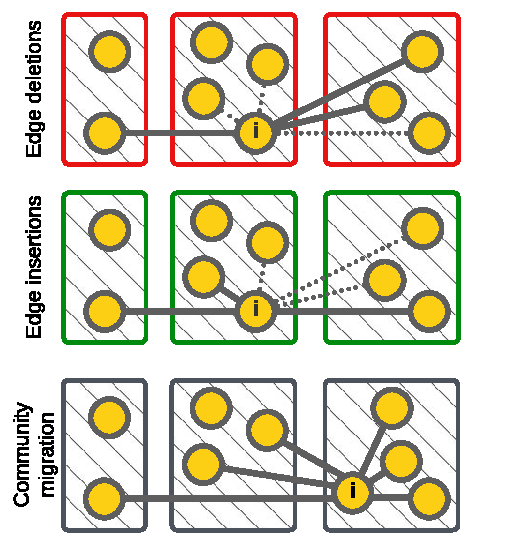
\includegraphics[width=0.3\linewidth]{out/about-cases-naive.pdf}
  }
  \subfigure{
    \label{fig:cases-delta-}
    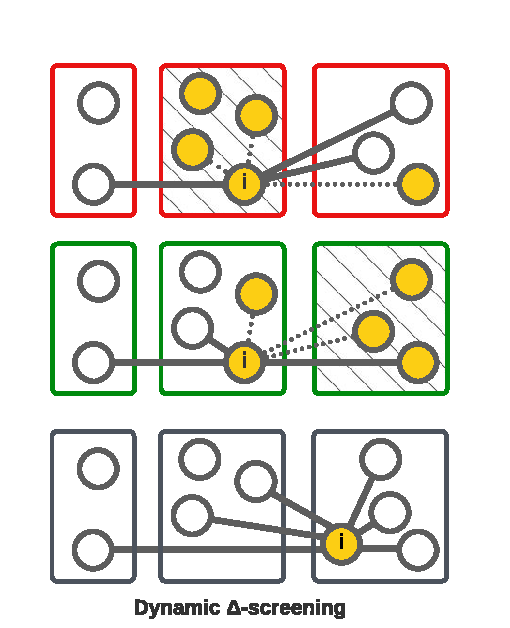
\includegraphics[width=0.3\linewidth]{out/about-cases-delta.pdf}
  }
  \subfigure{
    \label{fig:cases-frontier}
    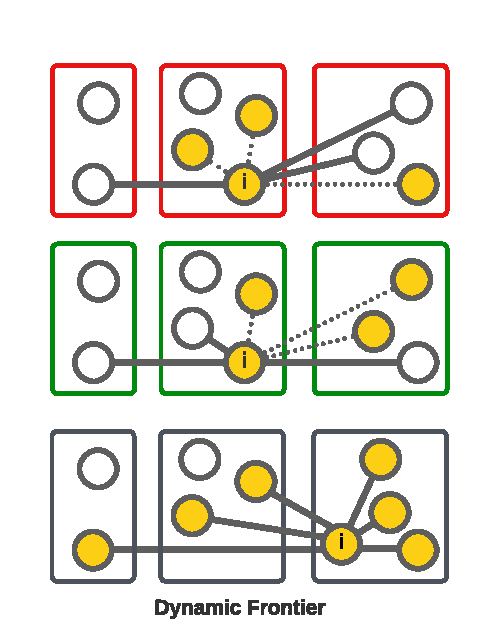
\includegraphics[width=0.3\linewidth]{out/about-cases-frontier.pdf}
  } \\[-2ex]
  \caption{Comparison of dynamic community detection approaches: \textit{Naive-dynamic} (\Nai{}), \textit{Dynamic $\Delta$-screening} (\Del{}), and \textit{Dynamic Frontier} (\Fro{}). Vertices marked as affected (initially) with each approach are highlighted in yellow, and when entire communities are marked as affected, they are hatched.}
  \label{fig:dynamic-approaches}
\end{figure*}

\begin{figure*}[!hbtp]
  \centering
  \subfigure[]{
    \label{fig:frontier-example-01}
    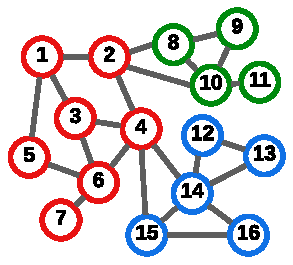
\includegraphics[width=0.18\linewidth]{out/about-frontier-01.pdf}
  }
  % \subfigure{
  %   \label{fig:frontier-example-02}
  %   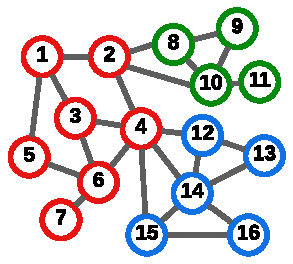
\includegraphics[width=0.15\linewidth]{out/about-frontier-02.pdf}
  % }
  \subfigure[]{
    \label{fig:frontier-example-03}
    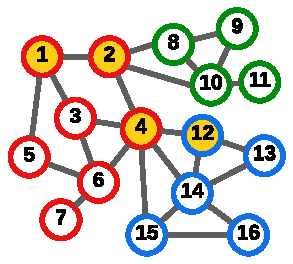
\includegraphics[width=0.18\linewidth]{out/about-frontier-03.pdf}
  }
  \subfigure[]{
    \label{fig:frontier-example-04}
    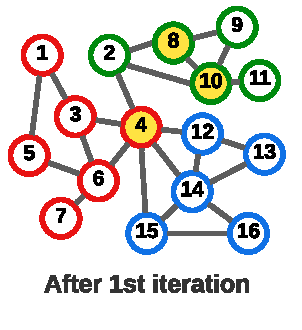
\includegraphics[width=0.18\linewidth]{out/about-frontier-04.pdf}
  }
  \subfigure[]{
    \label{fig:frontier-example-05}
    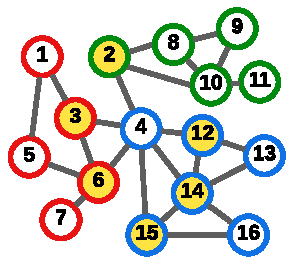
\includegraphics[width=0.18\linewidth]{out/about-frontier-05.pdf}
  }
  \subfigure[]{
    \label{fig:frontier-example-06}
    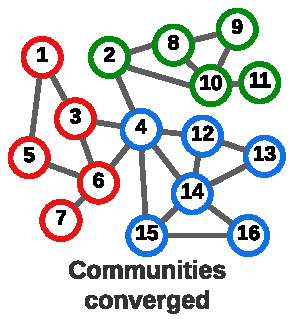
\includegraphics[width=0.18\linewidth]{out/about-frontier-06.pdf}
  } \\[-2ex]
  \caption{An example explaining the \textit{Dynamic Frontier} approach (\Fro{}). The community membership of each vertex is shown with border color (red, green, or blue), and the algorithm proceeds from left to right. A batch update arrives, affecting vertices $1$, $2$, $4$, and $12$. In the first iteration, vertex $2$ switches from red to green, impacting neighbors $8$ and $10$. In the second iteration, vertex $4$ changes from red to blue, affecting neighbors $3$, $6$, $12$, $14$, and $15$. Afterward, there are no more community changes.}
  % An example explaining the \textit{Dynamic Frontier} approach (\Fro{}). The community membership of each vertex is shown with border color (red, green, or blue), and the algorithm proceeds from left to right. \su{A batch update arrives, consisting of $\Delta^{t-}=\{(1, 2)\}$ and $\Delta^{t+}=\{(4, 12)\}$. Initially, \Fro{} marks vertices $1$, $2$, $4$, and $12$ as affected. In the first iteration, $2$ changes its membership from \textit{red} to \textit{green}, affecting neighbors $8$ and $10$. In the second iteration, $4$ changes its community from \textit{red} to \textit{blue}, affecting neighbors $3$, $6$, $12$, $14$, and $15$. Subsequently, no further community changes occur.
  \label{fig:frontier-example}
\end{figure*}


Given a batch update on the original graph, it is likely that only a small subset of vertices in the graph would change their community membership. Selection of the appropriate set of affected vertices to be processed (that are likely to change their community), in addition to the overhead of finding them, plays a significant role in the overall accuracy and efficiency of a dynamic batch parallel algorithm. Too small a subset may result in poor-quality communities, while a too-large subset will increase computation time. However, \Nai{} processes all the vertices, while \Del{} generally overestimates the set of affected vertices and has a high overhead. Our proposed \textit{Dynamic Frontier} approach (which we from here on refer to as \Fro{}) addresses these issues.


\subsubsection{Explanation of the approach}

We now explain \Fro{}. Consider a batch update consisting of edge deletions $(i, j) \in \Delta^{t-}$ and insertions $(i, j, w) \in \Delta^{t+}$, shown with double-dashed lines and double-solid lines respectively, with respect to a single source vertex $i$, in Figure \ref{fig:dynamic-approaches}. At the start of the community detection algorithm, we initialize the community membership of each vertex to that obtained in the previous snapshot of the graph.

\paragraph{Initial marking of affected vertices on edge deletion/insertion}

For edge deletions between vertices belonging to the same community and edge insertions between vertices belonging to different communities, we mark the source vertex $i$ as affected, as shown with vertices highlighted in yellow, in Figure \ref{fig:dynamic-approaches}. Note that batch updates are undirected, so we effectively mark both the endpoints $i$ and $j$. Edge deletions between vertices lying across communities and edge insertions for vertices lying within the same community are ignored (for reasons stated before).

\paragraph{Incremental marking of affected vertices on vertex migration to another community}

When a vertex $i$ changes its community during the community detection algorithm (shown with an arrow, with the direction indicating the migration of source vertex $i$ from its previous community to another new community), we mark all its neighbor vertices $j \in J_i$ as affected, as shown if Figure \ref{fig:dynamic-approaches} (highlighted in yellow), and mark $i$ as not affected. To minimize unnecessary computation, we also mark an affected vertex $i$ as not affected even if  $i$ does not change its community. We call this as the vertex pruning optimization. The process is akin to a graph traversal and continues until the communities have converged.

\paragraph{Application to the first pass of Louvain algorithm}

We apply \Fro{} to the first pass of \Lou{} algorithm (see Line \ref{alg:louvain--remark-pass} in Algorithm \ref{alg:louvain}), as with \Del{}. In subsequent passes, if the aggregation tolerance condition is not met (Line \ref{alg:louvain--aggregation-tolerance} in Algorithm \ref{alg:louvain}), all super-vertices are marked as affected and processed according to Louvain. This takes less than $14\%$ of total time, so we don't use \Fro{} to find affected super-vertices. The tolerance condition only fails in the case of large batch updates.


\subsubsection{A simple example}

Figure \ref{fig:frontier-example} shows an example of \Fro{}.

\paragraph{Initial communities}

The original graph comprises a total of $16$ vertices, which are divided into three communities, distinguished by the border colors of \textit{red}, \textit{green}, and \textit{blue} (see Figure \ref{fig:frontier-example-01}). This community membership information of each vertex could have been obtained by executing either the static or dynamic version of the \Lou{}/\LPA{} algorithm.

\paragraph{Batch update and Marking affected (initial)}

Subsequently a batch update is applied to the original graph (see Figure \ref{fig:frontier-example-03}), involving the deletion of an edge between vertices $1$ and $2$, and the insertion of an edge between vertices $4$ and $12$. Following the batch update, we perform the initial step of \Fro{}, marking endpoints $1$, $2$, $4$, and $12$ as affected. At this point, we are ready to execute the first iteration of a community detection algorithm.

\paragraph{After first iteration}

During the first iteration (see Figure \ref{fig:frontier-example-04}), the community membership of vertex $2$ changes from \textit{red} to \textit{green} because it exhibits stronger connections with vertices in the \textit{green} community. In response to this change, the \Fro{} incrementally marks the neighboring vertices of $2$ as affected, specifically vertices $8$ and $10$. Vertex $2$ is no longer marked as affected due to pruning.

\paragraph{After second iteration}

Let us now consider the second iteration (see Figure \ref{fig:frontier-example-05}). Vertex $4$ is now more strongly connected to the \textit{blue} community, resulting in a change of its community membership from \textit{red} to \textit{blue}. As before, we mark the neighbors of vertex $4$ as affected, namely vertices $12$, $14$, and $15$. Vertex $4$, once again, no longer marked as affected due to vertex pruning.

\paragraph{Communities converged}

In the subsequent iteration (see Figure \ref{fig:frontier-example-06}), no other vertices have a strong enough reason to change their community membership. At this point, when employing \Lou{}, the aggregation phase commences consolidating communities into super-vertices to prepare for the subsequent pass of the algorithm. However, when employing the \LPA{}, this marks the conclusion of the algorithm.

\begin{algorithm}[hbtp]
\caption{GVE-Louvain: Our parallel Louvain algorithm.}
\label{alg:louvain}
\begin{algorithmic}[1]
\Require{$G$: Input graph}
\Require{$C$: Community membership of each vertex}
\Require{$G'$: Input/super-vertex graph}
\Require{$C'$: Community membership of each vertex in $G'$}
\Require{$K'$: Total edge weight of each vertex}
\Require{$\Sigma'$: Total edge weight of each community}
\Ensure{$G'_{C'}$: Community vertices (CSR)}
\Ensure{$H_t$: Collision-free per-thread hashtable}
\Ensure{$l_i$: Number of iterations performed (per pass)}
\Ensure{$l_p$: Number of passes performed}
\Ensure{$\tau$: Per iteration tolerance}
\Ensure{$\tau_{agg}$: Aggregation tolerance}

\Statex

\Function{louvain}{$G$} \label{alg:louvain--begin}
  \State Vertex membership: $C \gets [0 .. |V|)$ \textbf{;} $G' \gets G$ \label{alg:louvain--initialization}
  \ForAll{$l_p \in [0 .. \text{\small{MAX\_PASSES}})$} \label{alg:louvain--passes-begin}
    \State $\Sigma' \gets K' \gets vertexWeights(G')$ \textbf{;} $C' \gets [0 .. |V'|)$ \label{alg:louvain--reset-weights}
    \State Mark all vertices in $G'$ as unprocessed \label{alg:louvain--reset-affected}
    \State $l_i \gets louvainMove(G', C', K', \Sigma')$ \label{alg:louvain--local-move}
    \If{$l_i \le 1$} \textbf{break} \Comment{Globally converged?} \label{alg:louvain--globally-converged}
    \EndIf
    \State $|\Gamma|, |\Gamma_{old}| \gets$ Number of communities in $C$, $C'$
    \If{$|\Gamma|/|\Gamma_{old}| > \tau_{agg}$} \textbf{break} \Comment{Low shrink?} \label{alg:louvain--aggregation-tolerance}
    \EndIf
    \State $C' \gets$ Renumber communities in $C'$ \label{alg:louvain--renumber}
    \State $C \gets$ Lookup dendrogram using $C$ to $C'$ \label{alg:louvain--lookup}
    \State $G' \gets louvainAggregate(G', C')$ \label{alg:louvain--aggregate}
    \State $\tau \gets \tau / \text{\small{TOLERANCE\_DROP}}$ \Comment{Threshold scaling} \label{alg:louvain--threshold-scaling}
  \EndFor \label{alg:louvain--passes-end}
  \State $C \gets$ Lookup dendrogram using $C$ to $C'$ \label{alg:louvain--lookup-last}
  \Return{$C$} \label{alg:louvain--return}
\EndFunction \label{alg:louvain--end}
\end{algorithmic}
\end{algorithm}

\begin{figure}[hbtp]
  \centering
  \subfigure{
    \label{fig:adjust-auxiliary--8020}
    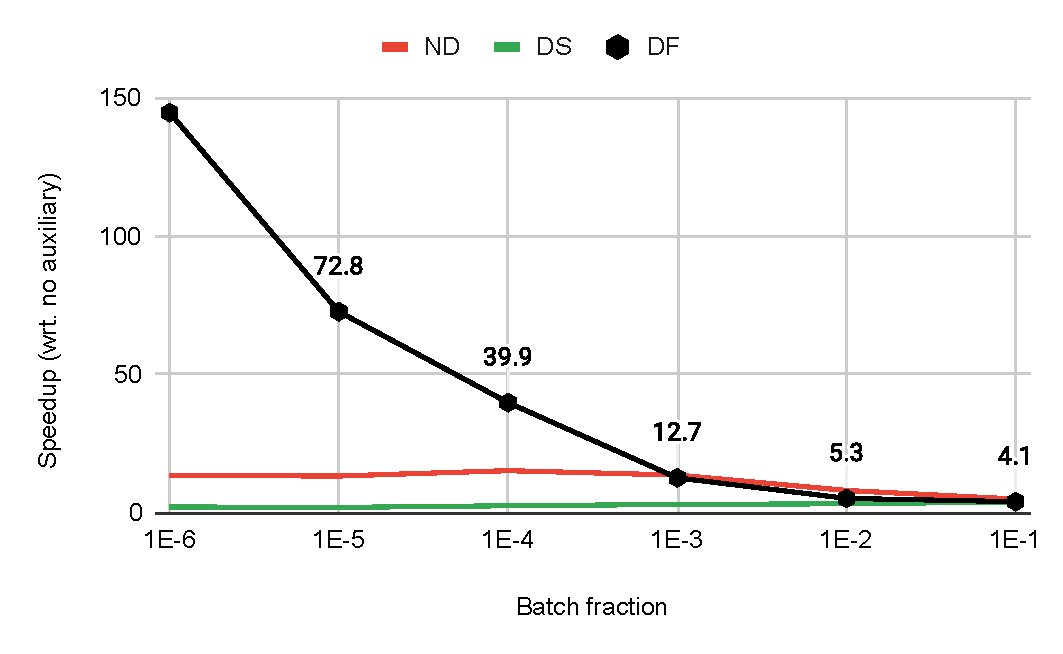
\includegraphics[width=0.98\linewidth]{out/adjust-auxiliary-8020.pdf}
  } \\[-2ex]
  \caption{Speedup of \textit{Naive-dynamic (ND)}, \textit{Delta-screening (DS)}, and \textit{Dynamic Frontier (DF)} Louvain when reusing the previous \textit{weighted-degrees of vertices} and \textit{total edge weight of communities} as auxiliary information to the dynamic algorithm, compared to the same dynamic algorithm when both are recomputed from scratch. This is done on large graphs with generated random batch updates of size $10^{-7} |E|$ to $0.1 |E|$\ignore{, consisting of $80\%$ edge insertions and $20\%$ deletions, to simulate realistic dynamic graph updates}.}
  \label{fig:adjust-auxiliary}
\end{figure}





\subsection{Our Dynamic Frontier based Louvain (\FroLou{}, Algorithm \ref{alg:louvain})}
\label{sec:dynamic-louvain}

We show how to apply our \textit{Dynamic Frontier} approach (\Fro{}) to \Lou{} in Algorithm \ref{alg:louvain} (which we call \FroLou{}). We take as input the previous snapshot of the graph $G^{t-1}$, the previous community membership of each vertex $C^{t-1}$, and the batch update consisting of edge deletions $\Delta^{t-}$ and insertions $\Delta^{t+}$ in Line \ref{alg:louvain--main-begin}. First, in Lines \ref{alg:louvain--restart-begin}-\ref{alg:louvain--restart-end}, we check if we should use \StaLou{} to maintain the quality of communities (explained in Section \ref{sec:restart}). Then, in Lines \ref{alg:louvain--mark-begin}-\ref{alg:louvain--mark-end}, based on \Fro{}, we mark the initial set of vertices as affected. In Lines \ref{alg:louvain--membership} and \ref{alg:louvain--super-membership-begin}-\ref{alg:louvain--super-membership-end}, we initialize the community membership of each vertex in the graph $G^t$, and each super-vertex in the aggregated graph $G'$ (in the first pass, this is the same as the input graph $G^t$).

For each pass (Lines \ref{alg:louvain--passes-begin}-\ref{alg:louvain--passes-end}), we perform the \textit{local-moving} phase of \Lou{} in Line \ref{alg:louvain--local-move}. If the community labels converge after one iteration, we terminate the algorithm (Line \ref{alg:louvain--globally-converged}). In Line \ref{alg:louvain--renumber}, we renumber the community-ids. This renumbering helps generate the aggregated graph $G'$ in the Compressed Sparse Row (CSR) format and counting the number of communities. In Line \ref{alg:louvain--lookup}, we update the community membership of each vertex $C$ based on the community membership of each super-vertex, such that we refer to the top-level hierarchy of the dendrogram as the final result.

Next, at Line \ref{alg:louvain--aggregation-tolerance}, we check whether only a small portion of communities have merged together. To do this, we calculate the ratio of the number of communities after the \textit{local-moving} phase $|\Gamma|$ to the original number of communities $|\Gamma_{old}|$. If this ratio $|\Gamma|/|\Gamma_{old}|$ is less than a specific value called the aggregation tolerance ($\tau_{agg}$, whose optimal value is measured and mentioned in Section \ref{sec:louvain}), it means that the merging has been minimal. In such a situation, we stop the algorithm to avoid the computationally expensive \textit{aggregation} phase, as it doesn't provide significant benefits. However, if a sufficiently large number of communities have merged together, we proceed with the \textit{aggregation} phase and obtain the aggregated graph $G'$. This graph is stored in CSR format.

Next, we perform the threshold scaling optimization \cite{com-naim17}, i.e., we reduce the tolerance $\tau$ by a tolerance drop factor of \verb|TOLERANCE_DROP|. This optimization helps minimize the number of iterations performed in the local-moving phase of \Lou{}. It improves performance with little sacrifice in the quality of communities obtained.

We now discuss the \textit{local-moving} phase of \Lou{}. First, in Lines \ref{alg:louvain--edge-weigths-begin}-\ref{alg:louvain--edge-weigths-end}, we calculate the total edge weights linked to each vertex $K'$ and the total edge weights linked to each community $\Sigma'$. For each iteration (Lines \ref{alg:louvain--iterations-begin}-\ref{alg:louvain--iterations-end}), and for each affected vertex $i$ in the graph $G'$, we use per-thread collision-free hashtables to obtain the best community linked to each vertex $c^*$, as well as the associated delta-modularity (highest) $\delta Q^*$ in parallel using Equation \ref{eq:delta-modularity} (Lines \ref{alg:louvain--best-community-begin}-\ref{alg:louvain--best-community-end}). If the best community $c^*$ is different from the original community membership $C'[i]$ of vertex $i$ (Line \ref{alg:louvain--best-community-same}), we update the community membership of the vertex and atomically update the total edge weights linked to each community in Lines \ref{alg:louvain--perform-move-begin}-\ref{alg:louvain--perform-move-end}. In addition, if this is the first pass of \Lou{} (Line \ref{alg:louvain--remark-pass}), based on \Fro{}, we mark the neighbors of vertex $i$ as affected in Line \ref{alg:louvain--remark}. To minimize unnecessary computation, we also mark vertex $i$ as not affected (whether or not $i$ changes its community) as part of vertex pruning optimization in Line \ref{alg:louvain--prune}. At the end of each iteration, if the total delta-modularity across all vertices $\Delta Q$ is less than the specified tolerance $\tau$, we terminate the local-moving phase (Line \ref{alg:louvain--locally-converged}). We prove the correctness of \FroLou{} in Section \ref{sec:louvain-correctness}.




\subsection{Maintaining quality across batches}
\label{sec:restart}

In our experiments with continuous batch updates of edge insertions of size $10^{-3} |E|$, we find that the quality of communities obtained using the \DelLou{} and \FroLou{} starts to drop (compared to \StaLou{}) by $48\%$ (rapid decline) and $5.7\%$ respectively after around $1300$ batches of updates. The same happens for \FroHyb{} by $10\%$ after around $600$ updates. Therefore, we conservatively use a \verb|RESTART_LOUVAIN| of $1000$, and a \verb|RESTART_HYBRID| of $500$ (see Lines \ref{alg:louvain--restart-begin}-\ref{alg:louvain--restart-end} in Algorithm \ref{alg:louvain}, and Lines \ref{alg:hybrid--restart-begin}-\ref{alg:hybrid--restart-end} in Algorithm \ref{alg:hybrid}). As the lines show, we run \StaLou{} once for $1000$/$500$ batches of updates to maintain the quality of communities across multiple batch updates and correct the error introduced. We adjust our reported timings by amortizing its cost.




\subsection{Time and Space complexity}
\label{sec:complexity}

To analyze the time complexity of our algorithms, we use $N_B$ to denote the number of vertices marked as affected (which is dependent on the size and nature of batch update) by the dynamic algorithm on a batch $B$ of edge updates, use $M_B$ to denote the number of edges with one endpoint in $N_B$, and $K$ to denote the total number of iterations performed. Then the time complexity of Algorithms \ref{alg:louvain}-\ref{alg:hybrid} is $O(K M_B)$. In the worst case, the time complexity of our algorithms would be the same as that of the respective static algorithms, i.e., $O(KM)$. The space complexity of our algorithms is the same as that of the static algorithms, i.e., $O(N + M)$.
